\begin{table}[htbp]
    \centering
    \caption[FACTS workload composition]{\captitle{FACTS workload composition.} Composition of workloads from the SPEC CPU 2006 benchmark suite for validating FACTS. The workloads were generated based on the method described in Section~\ref{section: workloads}.}
    \begin{tabular}{@{}lllr@{}}
        \toprule
        Workload & Set of benchmarks & Categories \\
                 &                   & (Section~\ref{section: workloads})\\
        \midrule
        8C   & Bzip2, Calculix, Gobmk, Soplex    & NNNT \\
             & CactusADM, Astar, Tonto, Povray   & FTNN \\
        2M6C & Astar, Calculix, CactusADM, Gobmk & TNFN \\
             & Soplex, Povray, Tonto, Bzip2      & TNNN \\ 
        4M4C & Astar, Milc, CactusADM, Lbm       & TSFF \\ 
             & Gobmk, Tonto, Povray, Bzip2       & NNNN \\ 
        6M2C & Xalancbmk, Wrf, GemsFDTD, Astar   & TSFF \\
             & Lbm, Tonto, Calculix, CactusADM   & FNNF \\ 
        8M   & Astar, Tonto, CactusADM, GemsFDTD & TNFT \\
             & Lbm, Milc, Bzip2, Mcf             & FSNS \\ 
        \bottomrule
\end{tabular}
    \label{tab: factsworkload}
\end{table}

\vspace{2em}

\section{Evaluation} 
\label{sec: evaluationreppc}

This section describes the workloads used to train and validate REPP-C. Next, we evaluate
FACTS against state-of-the-art schedulers and REPP-C.

\subsection{Workloads} 
\label{subsec: reppc workloads} 

In validating FACTS, we run \texttt{twice} as many threads as cores available, to
determine the effectiveness of the collocation technique.  In evaluating REPP-C, we launch
as many benchmark threads as cores available (as in prior
works~\citep{Su:2014:POP:2742155.2742200, Nishtala:SBACPAD, Nishtala:HPCA}).


\looseness -1 For each evaluation, we run several different combinations of workloads
concurrently; each workload is a mix of applications ranging from compute intensive to
memory intensive~\citep{2006core2}.  As in prior
work~\citep{Nishtala:2013:ETC:2555754.2555775, Zhuravlev:2013:SES:2498743.2498946,
Su:2014:POP:2742155.2742200, Zhuravlev:2012:SST:2379776.2379780,
Mars:2011:BIU:2155620.2155650, Mars:2011:DCC:1944862.1944887,
Gandhi:2010:OAE:1869138.1869264}, we select a subset of benchmarks from the SPEC suite to
represent the effectiveness of our technique.  The process of generating a multiprogrammed
workloads is described in section~\ref{section: workloads}. However, for REPP-C, we
categorise the workloads into two groups: the first group, compute intensive contains
workloads from insensitive (N) and Cache-Friendly (F); the second group, memory intensive
has workloads from Cache-Fitting (T) and Streaming/Thrashing (S).

Table~\ref{tab: factsworkload} shows the different workloads used in our experiment to
evaluate FACTS. In particular the workloads are: (\textsf{8C}) 8 compute intensive
threads, (\textsf{2M6C}) two memory and six compute intensive, (\textsf{4M4C}) four memory
and four processor intensive, (\textsf{6M2C}) six memory and four compute intensive and
(\textsf{8M}) 8 memory intensive workloads.

Table~\ref{tab: repworkload} refers to the workloads used in our environment for
validating REPP-C. In particular, the \textsf{\textbf{boldfaced}} workloads are used for
training the model: (\textsf{\textbf{4C}}) four compute intensive,
(\textsf{\textbf{2M2C}}) two memory-intensive and two compute-intensive,
(\textsf{\textbf{4M}}) four memory intensive. The remaining workloads are used for
validating: (\textsf{3C1M}) three compute- and one memory-intensive, (\textsf{1C3M}) one
compute-intensive and three memory-intensive, and (\textsf{4R1}, \textsf{4R2}) two
randomly chosen set of workloads consisting of four benchmarks each.  


\begin{table}[htbp] 
    \centering 
    \caption[REPP-C workload composition]{\captitle{REPP-C workload composition.} Composition of \textsf{\textbf{training}} and validation workloads from
    the SPEC CPU 2006 benchmark suite. The boldfaced workloads used as training workloads. The workloads were generated based on the method described in Section~\ref{section: workloads}.} 
    \begin{tabular}{@{}lllr@{}} 
        \toprule
        Workload & Set of benchmarks & Categories \\
                 &                   & (Section~\ref{section: workloads})\\ 
        \midrule 
        \textsf{\textbf{4C}} & Calculix, Gobmk, Bzip2, Tonto     & NNNN\\ 
        \textsf{\textbf{2M2C}} & Lbm, Astar, CactusADM, Calculix & FTFN\\ 
        \textsf{\textbf{4M}} & Astar, Mcf, Lbm, Milc             & TSFS\\ 
        3C1M & Povray, Bzip2, Calculix, Soplex                   & NNNT\\ 
        1C3M & Tonto, Lbm, Milc, Soplex                          & NFST\\ 
        4R1 & Astar, Bzip2, Mcf, Soplex                          & TNSS\\
        4R2 & Lbm, Bzip2, Calculix, GemsFDTD                     & FNNT\\ 
        \bottomrule 
    \end{tabular}
    \label{tab: repworkload} 
\end{table}


\subsection{Energy Efficient Scheduler} 
\label{subsec: facts}

We evaluate FACTS against two state-of-the-art algorithms:
DIO~\citep{Blagodurov:2010:CSM:1880018.1880019} and CFS. DIO is a thread scheduling
technique directed towards reducing contention for shared resource in components like
cache and memory. DIO dynamically schedules threads by spreading contention equally among
different memory domains, taking into consideration the cache intensity of the threads.
On the other hand, Linux scheduler time shares the core uniformly among all application
without considering the compute intensity or memory intensity of workloads. 


In evaluating FACTS, DIO and Linux scheduler, the active cores are set to all possible
combination of DVFS states in consecutive runs for each workload available. This process
is repeated across each scheduler consecutively. To compare the different scheduling
policies, we analyse the results obtained for the total energy efficiency, activity in LLC
and the total performance of all workloads for the \textsf{first 1000 seconds} of
execution of the workload. Also, we study the pair of threads that are executed on a given
core at a particular DVFS state. 


Previous research~\citep{Nishtala:2013:ETC:2555754.2555775,
Zhuravlev:2013:SES:2498743.2498946,Blagodurov:2010:CSM:1880018.1880019,
Zhuravlev:2012:SST:2379776.2379780, Becchi:2006:DTA:1128022.1128029} has shown that
contention for shared resources in cache hierarchy can impact performance of the threads
drastically. Miss penalty, measured in computational cycles, is defined as the ratio of
memory access time to the inverse of frequency. Therefore, the power consumption increases
as miss penalty to access the lower levels of caches increase.  

\iffalse
\begin{figure*}[tb!]
   \centering
    \begin{subfigure}{.5\textwidth}
        \centering
        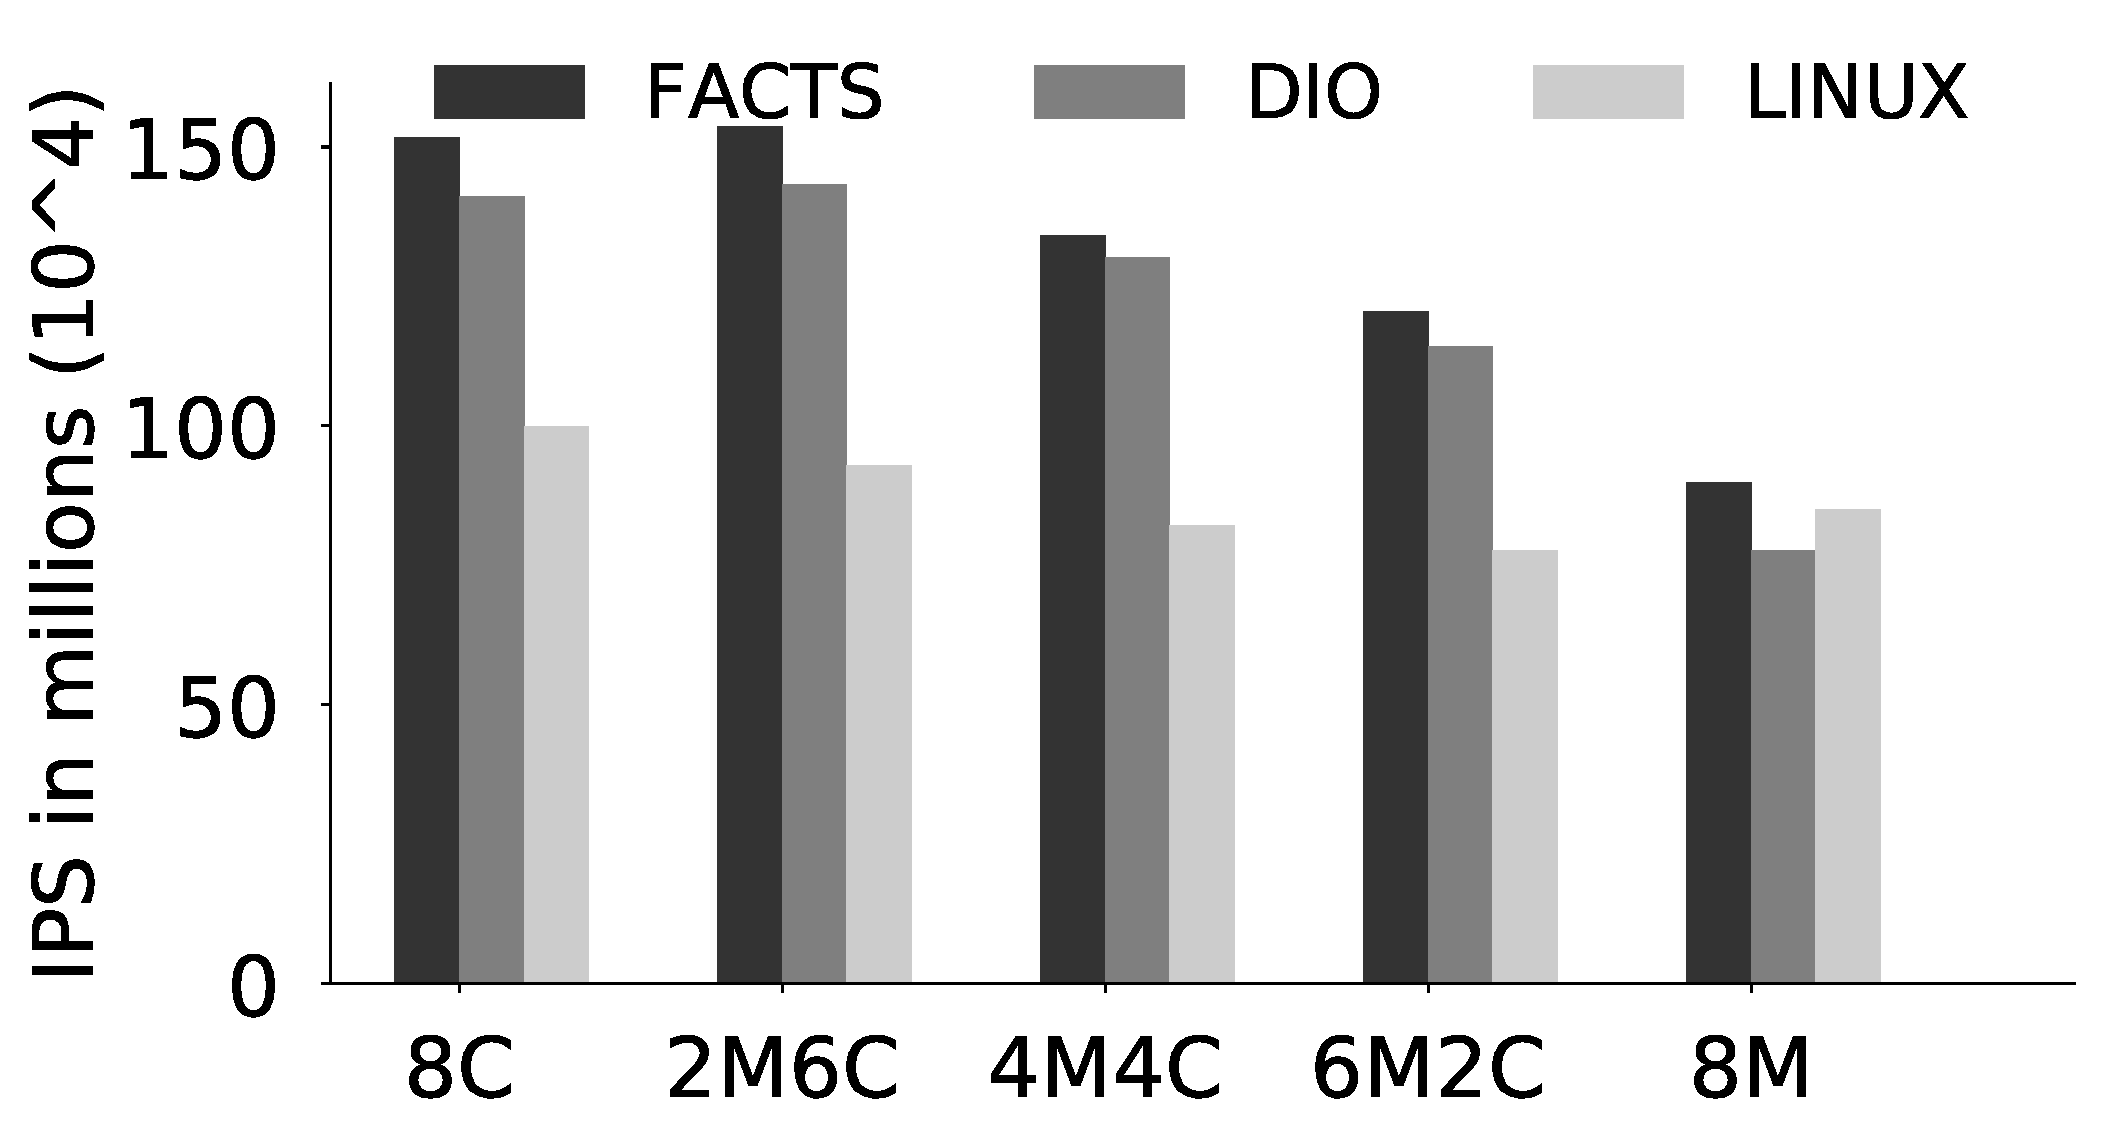
\includegraphics[width=\textwidth]{Chapter3/Figs/consolidation/perf.eps}
        \caption{Performance (MIPS)}
        \label{fig: perfmips}
    \end{subfigure}
    \begin{subfigure}{0.5\textwidth}
        \centering
        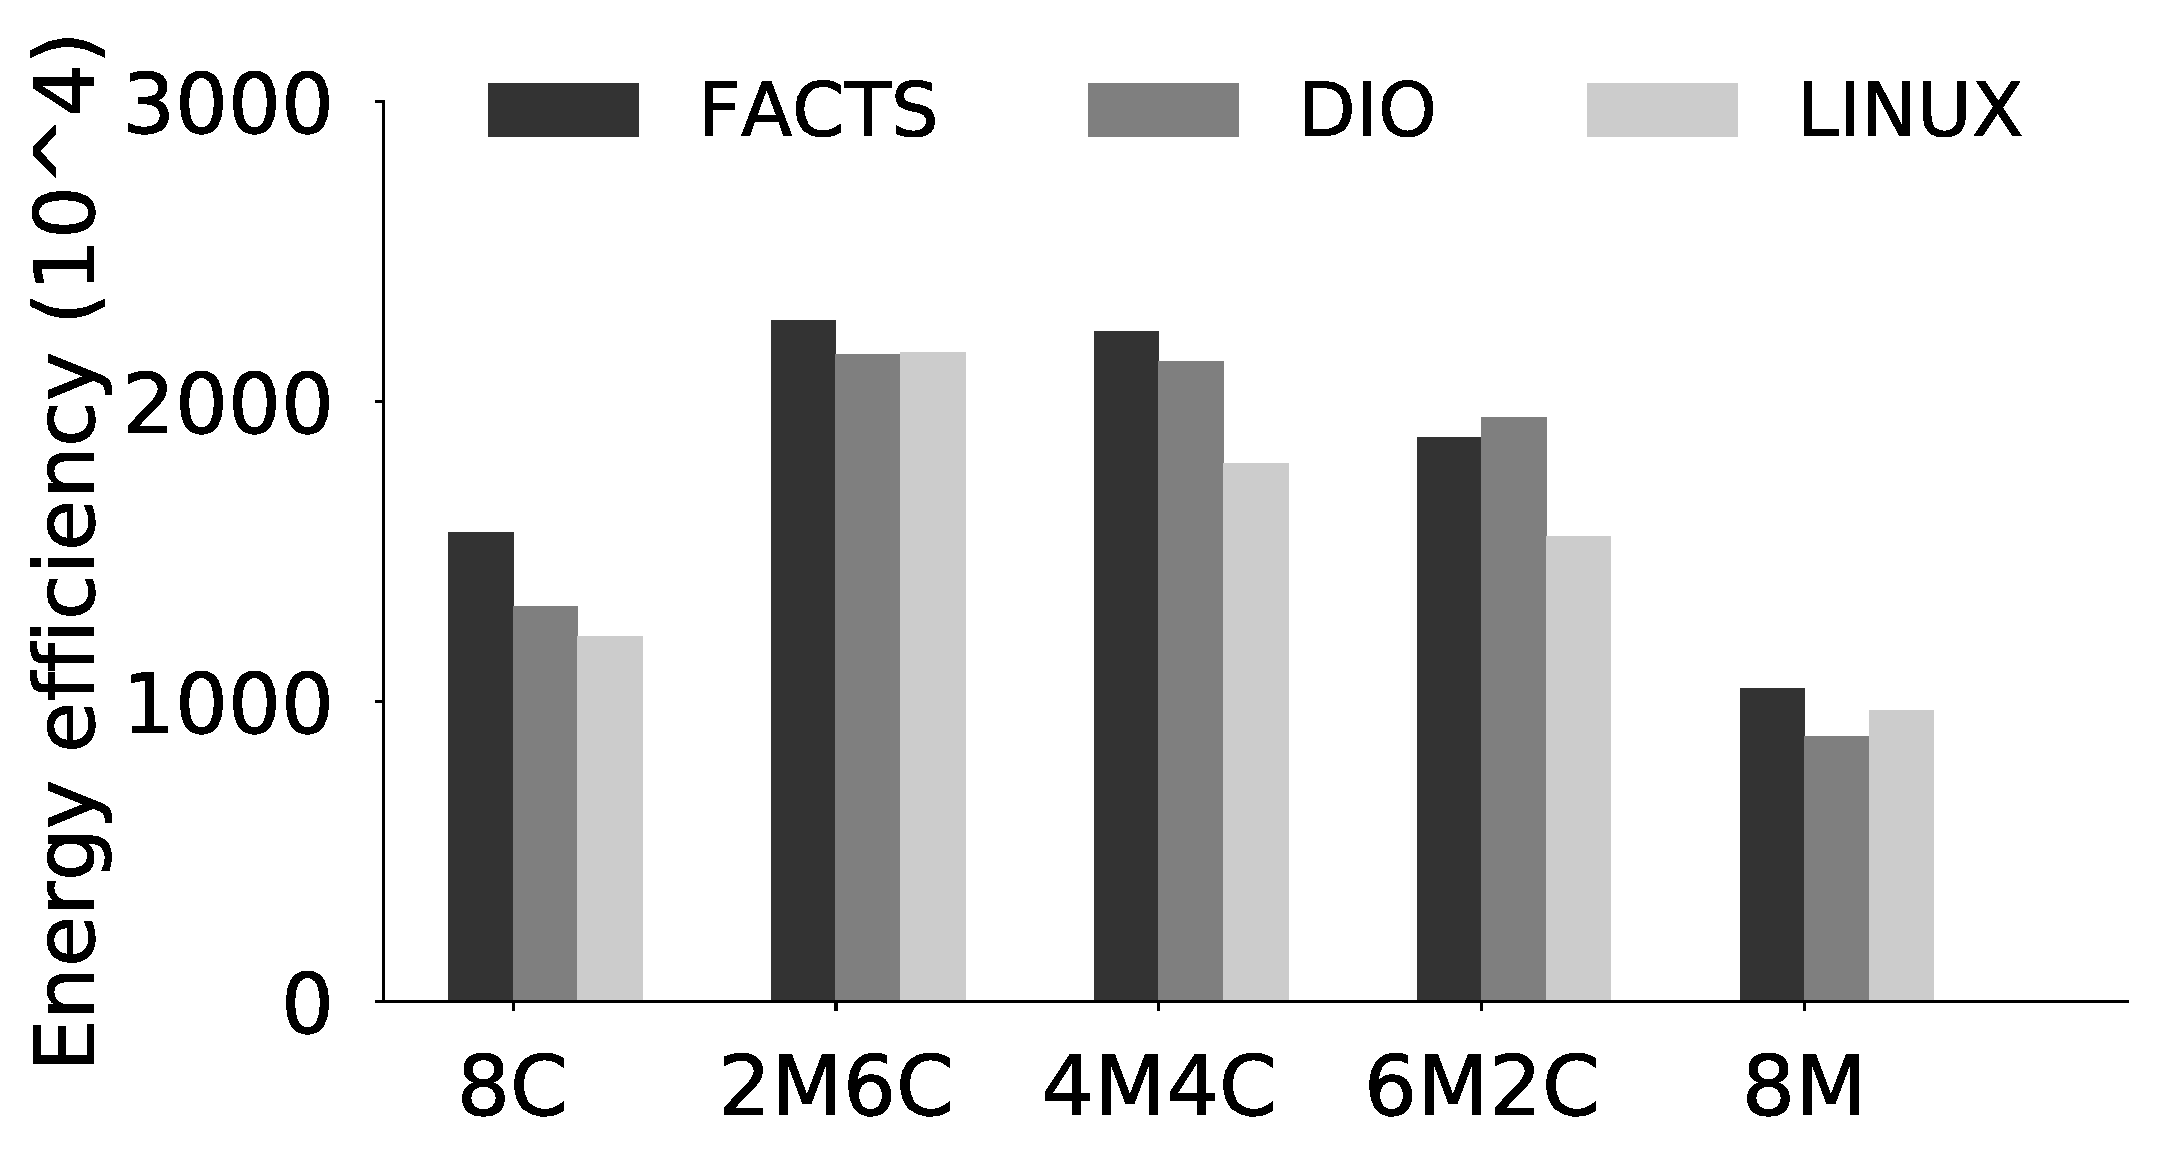
\includegraphics[width=\textwidth]{Chapter3/Figs/consolidation/ef.eps}
        \caption{Energy efficiency (MIPS/Watt)}
        \label{fig: Energy Efficiency}
    \end{subfigure}%
    \begin{subfigure}{0.5\textwidth}
        \centering
        \includegraphics[width=\textwidth]{Chapter3/Figs/consolidation/llc.eps}
        \caption{LLC misses}
        \label{fig: LLC}
    \end{subfigure}
    \caption[Performance evaluation for FACTS against DIO and Linux]{\captitle{Performance evaluation for FACTS against DIO and Linux.} Performance (\ref{fig: perfmips}), Energy efficiency (\ref{fig: Energy Efficiency}) and LLC misses (\ref{fig: LLC}) for all workloads over all frequency set combinations for \textit{FACTS}, \textit{DIO} and Linux scheduler with eight threads.}
    \label{fig: FACTS result}
\end{figure*}
\fi


Specifically, we show three main reasons why FACTS improves over DIO and Linux in
performance and energy efficiency when run for a fixed time quantum of \SI{1000}{\second}.
First, one might intuitively assume FACTS runs slower because it has a higher number of
thread migrations which might cause high overhead and make the workloads take longer when
dynamically mapped between cores, thus having less performance.  Towards that,
Figure~\ref{fig: perfmips} shows that the total performance of FACTS improves over DIO by
\SI{8.25}{\percent} (mean) and Linux by \SI{37.56}{\percent} (mean).  Second, since FACTS
runs threads faster than DIO, we assume that it might have a higher energy consumption.
However, FACTS schedules workloads based on the demand for memory bandwidth and core DVFS states.
Therefore, the threads which stall for memory are migrated to cores with lower

\begin{wrapfigure}{r}{0.5\textwidth}
   \centering
    \vspace{-4mm}
    \begin{subfigure}{.5\textwidth}
        \centering
        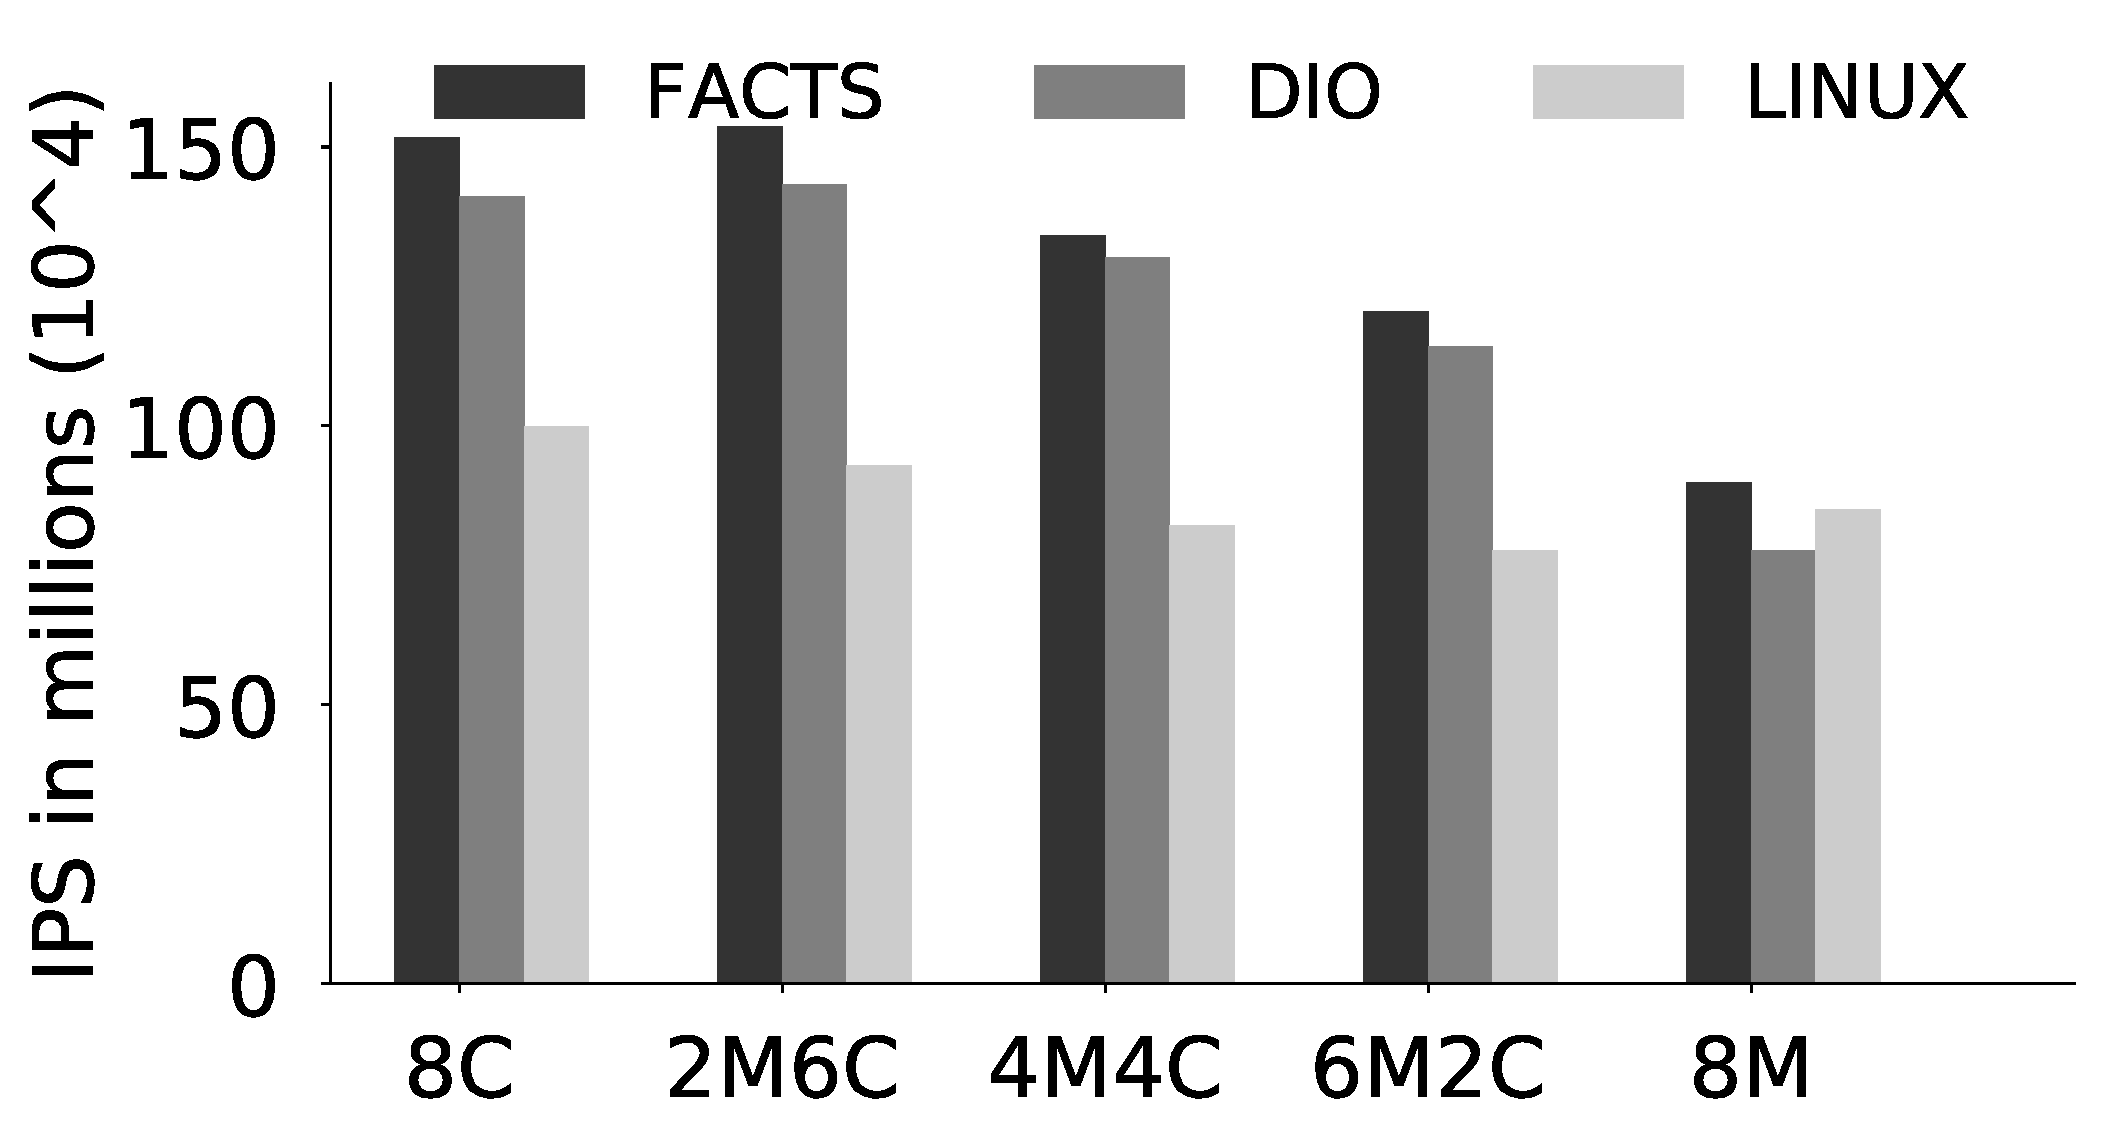
\includegraphics[width=\textwidth]{Chapter3/Figs/consolidation/perf.eps}
        \caption{Performance (MIPS)}
        \label{fig: perfmips}
    \end{subfigure}
    \begin{subfigure}{0.5\textwidth}
        \centering
        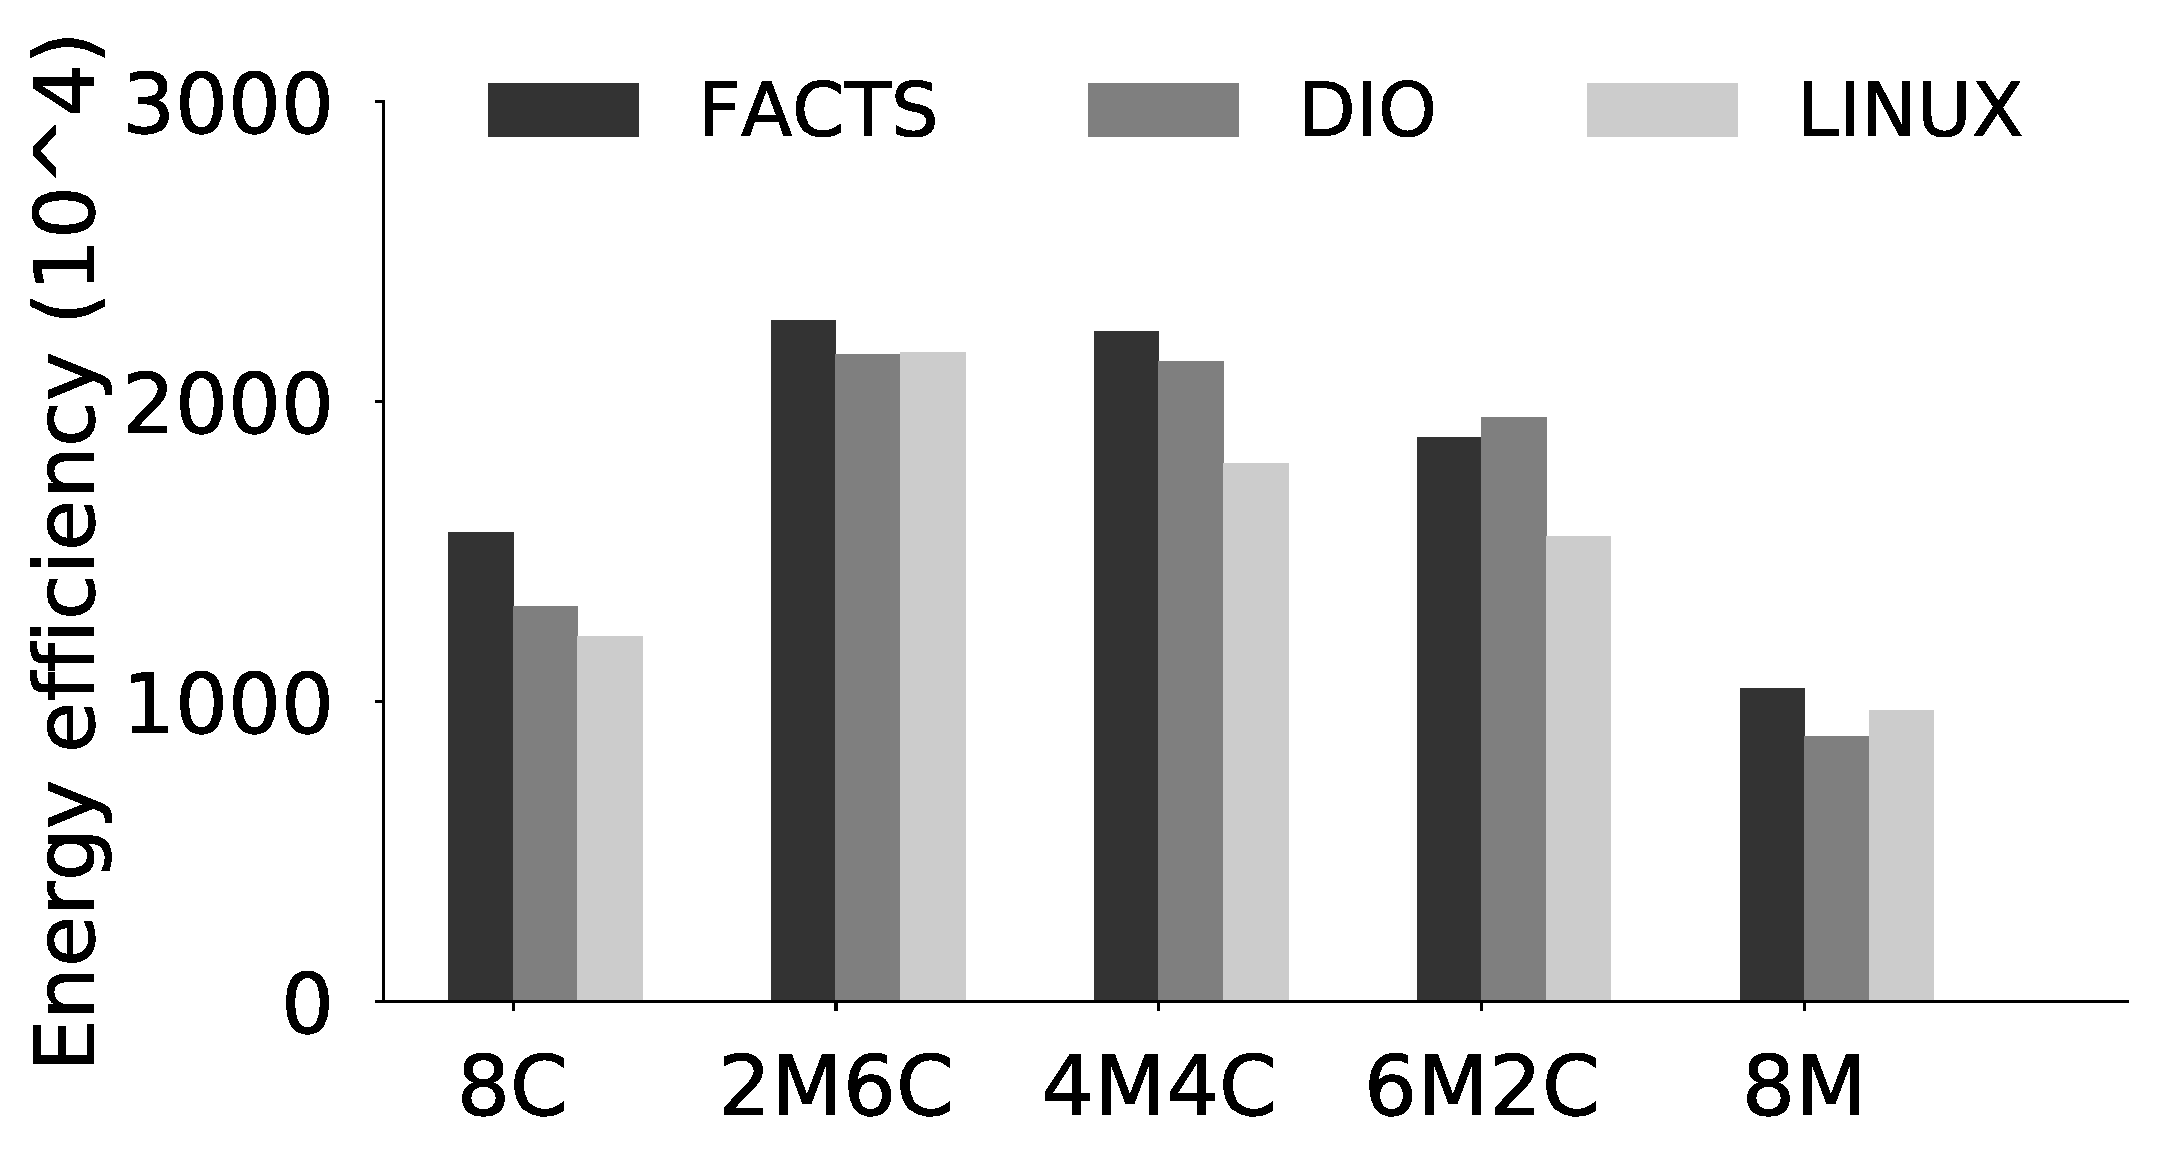
\includegraphics[width=\textwidth]{Chapter3/Figs/consolidation/ef.eps}
        \caption{Energy efficiency (MIPS/Watt)}
        \label{fig: Energy Efficiency}
    \end{subfigure}
    \begin{subfigure}{0.5\textwidth}
        \centering
        \includegraphics[width=\textwidth]{Chapter3/Figs/consolidation/llc.eps}
        \caption{LLC misses}
        \label{fig: LLC}
    \end{subfigure}
    \caption[Performance evaluation for FACTS against DIO and Linux]{\captitle{Performance evaluation for FACTS against DIO and Linux.} Performance (\ref{fig: perfmips}), Energy efficiency (\ref{fig: Energy Efficiency}) and LLC misses (\ref{fig: LLC}) for all workloads over all frequency set combinations for \textit{FACTS}, \textit{DIO} and Linux scheduler with eight threads.}
    \label{fig: FACTS result}
    \vspace{2mm}
\end{wrapfigure}


\noindent DVFS state, thus resulting in a small idle time for compute intensive threads and small
power consumption while stalling for memory. Towards that, we looked at the energy
efficiency (MIPS/watt -- performance/watt) and show that FACTS improves over DIO by
\SI{6.2}{\percent} (mean) and Linux by \SI{14.17}{\percent} (mean) (see Figure~\ref{fig:
Energy Efficiency}). Third, since FACTS migrates threads which stall for memory to cores
with lower DVFS state, and DIO does not, it improves the performance of the co-scheduled
threads and reduces the LLC misses by \SI{4.87}{\percent} (mean) over DIO and
\SI{41.70}{\percent} (mean) over Linux (see Figure~\ref{fig: LLC}).



In addition, while executing workload 4M4C at DVFS states \SI{1.6}{\giga\hertz},
\SI{2.4}{\giga\hertz}, \SI{0.8}{\giga\hertz} and \SI{0.8}{\giga\hertz} on cores 0-3,
respectively.  DIO schedules \emph{cactusADM} and \emph{Tonto} on core with DVFS state
\SI{0.8}{\giga\hertz} for \SI{82}{\percent} of the execution time. We note that
\emph{cactusADM} is a mid memory intensive, whereas, \emph{Tonto} has low memory activity.
On the other hand, FACTS schedules the pair of threads, \emph{Astar} and \emph{Bzip2} are
allocated for \SI{10.65}{\percent}; \emph{Astar} and \emph{cactusADM} for
\SI{15.2}{\percent}; \emph{Bzip2} and \emph{cactusADM} are allocated for
\SI{74.15}{\percent} of the execution time on the core with DVFS state
\SI{0.8}{\giga\hertz}.  Specifically in this scenario, we improve over DIO by
\SI{6.84}{\percent} in performance.


\subsection{Multicore Models including Consolidation with Constraints}%REPP-C}
\label{subsec: evalREPP-C}

In validating REPP-C, we launch the multiprogrammed workloads consecutively using FACTS,
and show an example of the prediction technique to satisfy the constraints (see
section~\ref{subsubsec: experiments repph}). The constraints are satisfied by selecting a
configuration from either REPP or REPP-C as described in section~\ref{subsec:
repporreppc}.

\begin{figure}[t]
    \centering
    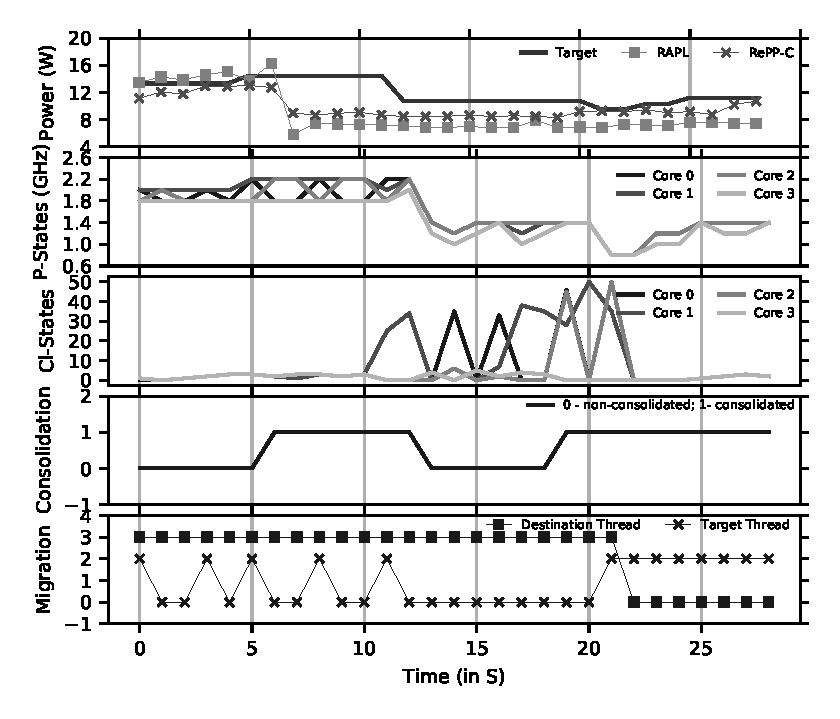
\includegraphics[scale=0.9]{Chapter3/Figs/consolidation/4r1-random.eps}
    \caption[Power prediction for a random workload]{\captitle{Power prediction for random workload.} Runtime view of the power prediction for workload 4R1 under change\_factor Randomised. In the bottom graph, destination and target threads refer to the thread with the least number and highest number of LLC misses, respectively. The numbers on the $y$-axis, in the last subplot, represent the threads in the same order as in Table~\ref{tab: repworkload}.}
    \label{fig: power realtime}
\end{figure}

Figure~\ref{fig: power realtime} shows an example of the power prediction technique
implemented on our system for the first 20 seconds of execution for the workload 4R1 with
constraint Random. From top-to-bottom, the first graph represents the power as measured
using RAPL, constraint (\textsf{Target}) and the prediction made using REPP-C. The second
and third graph show the changes in DVFS states, Cl-States for all cores in response to
changes in constraint along the course of the execution. The fourth graph shows, if REPP
(\textsf{non-consolidated}) or REPP-C (\textsf{consolidated}) is deployed.  Finally, the
fifth graph shows the co-runners for the three active cores for REPP-C and four active
cores for REPP. The numbers on the $y$-axis, in the last subplot, represent the threads in
the same order as in Table~\ref{tab: repworkload}.  We highlight two results. First,
REPP-C does show the capability to adapt to workloads consisting of multiple thread
phases~\citep{2006core2}, and ensure constraints per-thread are met with low error.
Despite the fact that there are phases where REPP-C have relatively higher error, for
instance, in seconds 7-10 REPP-C makes a \SI{3.6}{\watt} error, the average error is as
low as 4.03\%. Second, REPP-C and REPP can predict power per thread which native RAPL or
PEPP~\citep{Su:2014:POP:2742155.2742200} cannot achieve. This shows that the model is
accurate enough to capture the real behaviour, is driven by existing performance counters,
and, since the computational complexity at runtime is low, it can be used for fine-grain
power management. 

\begin{figure}[t]
   \centering
    \includegraphics[width=\textwidth]{Chapter3/Figs/consolidation/final-power.eps}
    \caption[Power prediction for multiprogrammed workloads with REPP-C]{\captitle{Power prediction for multiprogrammed workloads with REPP-C.} \textbf{Energy consumed (\SI{}{\milli\joule})} across all workloads under change\_factors High, Mid, Low and Random. The $y$-axis is read as MEASURED \textit{using RAPL} and constraint over time (\textit{Target})}.
    \label{fig: power workloads}
\end{figure}

Figure~\ref{fig: power workloads} shows the energy consumption in millijoules
(\SI{}{\milli\joule}) using the power \textsf{measured} using native RAPL register and
constraint over time (\textsf{Target}) for four workloads under all constraints (for all
load\_change and change\_factor) in period of 100 seconds. The $x$-axis represents the
type of workload, change\_factor and the load\_change interval (in seconds). The
configuration to satisfy the target is selected using REPP-C. 

The energy consumption target is measured as the summation of $\chi(\kappa)$ (as given by
Equation~\ref{eq: eachterm}).  On average, for all workloads, in under different
constraint, REPP-C exhibits an error in prediction of 7.55\% or \SI{115.67}{\milli\joule}.
Observe, that the maximum error we incur is \SI{286.4}{\milli\joule} (in 3C1M-Low\_6).
Moreover, the error in achieving the given energy target for change\_factors High, Mid,
Low and Random are \SI{217.22}{\milli\joule} (16.23\%), \SI{41.63}{\milli\joule} (2.24\%),
\SI{107.80}{\milli\joule} (5.69\%) and \SI{56.72}{\milli\joule} (3.02\%) respectively. 


\begin{figure}[t]
   \centering
    \includegraphics[width=\textwidth]{Chapter3/Figs/consolidation/final-perf.eps}
    \caption[Perfomance prediction for multiprogrammed workloads with
    REPP-C]{\captitle{Performance prediction for multiprogrammed workloads with REPP-C.}
    \textbf{Total performance (in Thousands)} across all workloads under change\_factors
    High, Mid, Low and Random. The $y$-axis is read as MEASURED \textit{using PMCs} and
    constraint over time (\textit{Target})}.  

    \label{fig: perf workloads} \end{figure}

Figure~\ref{fig: perf workloads} shows the total performance (MIPS) in thousands
\textsf{measured} using PMCs and the constraint over time (\textsf{Target}) for four
workloads under all constraints for a period of 100 seconds. The $x$-axis represents the
type of workload, change\_factor and the load\_change interval (in seconds). The
configuration to satisfy the target is selected using REPP-C.  The total performance
target is measured as the summation of $\chi(\kappa)$ (as given by Equation~\ref{eq:
eachterm}). We incur an average error of 8.96\% and a maximum error of 46.91\% (in
4R2-High\_9) and a total of \SI{206.19}{MIPS}.  Similar to the energy consumption target,
the total performance target is also measured.

Figure~\ref{fig: power workloads} and~\ref{fig: perf workloads} demonstrate that REPP-C
has been validated under multiple constraints, where each bar in the histogram represents
a summary of the workload execution, similar to Figure~\ref{fig: power realtime}.

\newpage
% Scalability & Implementation 
\section{Implementation of the Modelling and Prediction Technique}%REPP, REPP-H, and REPP-C} 
\label{subsec: implementation-REPPC}

%{\small \circled{a}} Gather offline traces and generate the power and performance models.  

REPP and REPP-C are user-level processes running on Linux OS that consist of four main
functions: {\small \circled{a}} Gather performance statistics (Section~\ref{sec: perfmon
thesis}), power meter readings (Section~\ref{sec: power meters}), and verify core's sleep
state residency.  {\small \circled{b}} Bind tasks-to-cores.  {\small \circled{c}} Predict
performance and power at each DVFS state and Cl-State (with and without core
consolidation).  {\small \circled{d}} Given a constraint, set DVFS state and Cl-State.  

\looseness -1 We set all inactive cores to the lowest DVFS state and facilitate the core to enter the
deepest sleep state. To verify the C-State residency (at sleep states \textsf{C3},
\textsf{C5}, and \textsf{C7}) during core consolidation, the MSR registers~\citep{Intel}
\textsf{MSR\_PKG\_C3\_RESIDENCY}, \textsf{MSR\_PKG\_C6\_RESIDENCY} and
\textsf{MSR\_PKG\_C7\_RES\-}\textsf{IDENCY} are read every
\SI{250}{\milli\second} on the Intel processor. The default time quantum to \textsl{enter}
a C-State is \SI{1024}{\nano\second}.

\looseness -1 In the process of generating the models, we bind tasks to cores via the
Linux \textsf{sched\_setaffinity} system call. Binding a task to a core ensures that the
thread runs on the specified core. Assigning the affinity~\citep{LinuxKernel} for a thread
bypasses Linux CFS and helps avoid excessive thread migration and provides a more controlled
environment.  The process of model generation is automatised using an R script in order to
be applicable systematically. This is feasible because no manual training is required,
showing that with a random set of benchmarks it is possible to generate accurate
performance and power models. 

The frequency scaling was performed by setting the \textit{CPUFreq governor} to
\textit{userspace} and scaling the frequency for individual cores (Kasture
\etal~\citep{Kasture2015Rubik} show that changes in DVFS are in the order of
microseconds). On the Intel processor, the MSR register
\textsf{MSR\_IA32\_PERF\_CTL}~\citep{acpikernel, Intel} is used to reduce the latency to a
single register move. Switching DVFS state using the MSR register overrides the Linux
kernel driver \textsf{acpi-cpufreq}. Next, the Cl-State are set using the Intel powerclamp
driver~\citep{powerclamp}.   


%\subsection{Algorithm Configuration} 

\paragraph{Algorithm Configuration.} A sampling interval of \SI{250}{\milli\second} was empirically chosen for
all phases of the algorithm i.e., to generate traces, build models and deploying REPP,
REPP-C, and FACTS.


%\subsection{Scalability}
%\label{section: scalability}

\paragraph{Scalability.} Scalability of a prediction algorithm is determined by the computational latency to make
predictions and the prediction accuracy. To visualise the scalability impact, we breakdown
the computational cost (in cycles) only for the Intel processor\footnote{We do not expect
the computational cost to have a large deviation across processors, as the technique
involves only a few mathematical operations and one I/O operation}, using the
\textsf{RDTSC}~\citep{RDTSC} instruction for the following computations: {\small
\circled{1}} Cost to read PMCs and compute ARs; {\small \circled{2}} Predicting
performance and power at all configuration without consolidation (REPP); {\small
\circled{3}} Predicting performance and power with consolidation (REPP-C); {\small
\circled{4}} Selecting REPP or REPP-C; {\small \circled{5}} Moving to a given
configuration. The estimates of computational overheads provided are recorded per
evaluation, and is the mean over multiple iterations.

The possible number of configuration on a four core system are 80 billion (450
configuration per core for REPP and REPP-C).  However, the overlap in performance and
power prediction over these configurations leads to redundancy in computational resources
and power. Therefore, we compute only 3600 configurations on a four core system running
both REPP and REPP-C.  Despite predicting only~\SI{0.5}{\percent} of the total number of
configuration possible, our results have shown that the estimation technique can predict
performance and power with an accuracy greater than \SI{93}{\percent}.  


\begin{figure}[t]
    \centering
\begin{tikzpicture}
[
    pie chart,
    slice type={comet}{blu},
    slice type={legno}{rosso},
    slice type={yel}{giallo},
    slice type={sedia}{viola},
    slice type={caffe}{verde},
    pie values/.style={font={\small}},
    %legend style={{font=\normalsize}},
    scale=3.5
]

    \pie[xshift=0.5cm,values of coltello/.style={pos=1.1}]%
        {Computational cost in cycles}{78.49/caffe,8.72/yel,4.36/sedia,7.27/comet,1.16/legno}

    %\legend[shift={(2cm,0.5cm)}]{{FACTS (3000 cycles)}/sedia, {Gathering PMCs (54000 cycles)}/caffe}
    \legend[shift={(2cm,1.0cm)}]{{FACTS (3000 cycles)}/sedia, {Gathering PMCs (54000 cycles)}/caffe, {Computing AR and predictions (6000 cycles)}/yel, {Consolidation model (5000 cycles)}/comet, {Select REPP or REPP-C (800 cycles)}/legno}

\end{tikzpicture}
    \caption[Scalability of REPP and REPP-C]{\captitle{Scalability of REPP and REPP-C.} The computational overhead measured in cycles (using \textsf{RDTSC}
     instruction) on the Intel processors is 68880 cycles.} 
    \label{fig: scalability} %
\end{figure}


\looseness -1 Figure~\ref{fig: scalability} shows the computational overhead (per
computation) when predicting performance and power on a four core system running at
\SI{2.4}{\giga\hertz}.  The total overhead is measured in cycles using the \textsf{RDTSC}
instruction is 68800 cycles.  The major overhead (54000 cycles) is due to the low level
operations to gather PMCs using \textsf{perf}. Next, computing the activity ratio and
predicting performance and power (6000 cycles).  Thereafter, selecting a potential
corunners using FACTS (3000 cycles), and applying the consolidation model (5000 cycles).
Finally, to select REPP or REPP-C and applying a given configuration (800 cycles). In
summary, it takes under 100 cycles per prediction of performance or power.

\begin{table}[t]
\centering
    \caption[Time complexity in predictions]{\captitle{Time complexity in predictions.} Number of configurations possible per core given the number of cores and time for modelling}
\begin{tabular}{@{}lrrrcrrrc@{}}\toprule
 $DVFS\enspace state$   & \multicolumn{3}{c}{$\SI{2.4}{\giga\hertz}$} & \phantom{abc}& \multicolumn{3}{c}{$\SI{0.8}{\giga\hertz}$} \\
\cmidrule{2-4} \cmidrule{6-8} 
    $Time(s)/\#cores $ & $1$ & $2$ & $4$ && $1$ & $2$ & $4$\\
\midrule
            \SI{0.500}{\second}   &900&230888&230888 &&900&76964&76964 \\ 
            \SI{0.250}{\second}   &900&115444&115444 &&900&38482&38482 \\ 
            \SI{0.125}{\second}   &900&57722&57722   &&900&19241&19241 \\ 
            \SI{0.063}{\second}   &900&29092&29092   &&900&9697&9697 \\ 
            \SI{0.031}{\second}   &900&14315&14315   &&900&4772&4772 \\ 
            \SI{0.016}{\second}   &900&7388&7388     &&900&2463&2463 \\ 
            \SI{0.008}{\second}   &900&3694&3694     &&900&1231&1231 \\ 

\bottomrule
\end{tabular}

\label{tab: coretime}
\end{table}

Table~\ref{tab: coretime} shows number of configurations that can be computed within a
given time quantum (measured in seconds) at \SI{2.4}{\giga\hertz} and
\SI{0.8}{\giga\hertz} on a machine with one, two, and four cores. For instance, the number
of configurations on a two core system are 810000. Nevertheless, given a DVFS state (say
\SI{2.4}{\giga\hertz}) and a time constraint (\SI{0.125}{\second}), the number of
predictions that can be computed are 57722, instead of 810000. Also observe that on a
machine with a single-core at \SI{2.4}{\giga\hertz} and \SI{0.8}{\giga\hertz}, the number
of configurations are the same because, irrespective of the DVFS state the number of
configurations are fixed at 450 per core for REPP and REPP-C.

Given the computational overhead, we suggest that our prediction methodology has minimal
overhead and is fine-grained. This enables REPP to characterise workload at a per thread
level using existing hardware counters to meet various constraints.
\newpage




\section{Conclusion}
\label{sec: reppcconclusion}

In this chapter, we presented REPP-C, a power and performance estimation model
parametrised by the hardware DVFS states, Cl-States, and core consolidation.  The
technique includes a systematic method to build models to predict performance and power
for each core, based on PMCs, and multi linear regression.  In the \muc environment with
consolidation, the \muc models are complemented by a correction to account for the impact
of consolidation. REPP-C implements a scheduling technique to place the threads which were
allocated on the consolidated core. 

\looseness -1 To allocate threads from the consolidated core to another one, we designed
Frequency, and Contention-Aware Thread mapping Schema (FACTS). FACTS is an online
frequency and contention-aware thread-to-core mapping scheduling policy for \muc systems.
FACTS can be implemented on any \muc processor without knowledge of the workload or the
target system.  Therefore, it is quick and easy to implement user-level Linux scheduler.
We compared FACTS with other state-of-the-art schedulers and our results show improvements
over all SPEC CPU 2006 workloads. FACTS improves energy efficiency by \SI{6.2}{\percent}
and \SI{14.2}{\percent} over DIO and native Linux scheduler, respectively.

FACTS is integrated in REPP-C to predict performance, and power with workload
consolidation. REPP-C's predictions are used to meet user specified constraints for
multiprogrammed workloads on \muc architectures. Our results show average errors of
\SI{7.55}{\percent} and \SI{8.96}{\percent} (with \SI{95}{\percent} confidence interval)
are observed when predicting energy and performance, respectively for numerous
multiprogrammed workloads. \newline
